\chapter{Historia madżonga}
% %%%%%%%%%%%%%%%%%%%%%%%%%%%%%%%%%%%%%%%%%%%%%%%%%%%%%%%%%%%%%%%%%%%%%%%%
% DEFINICJE
% %%%%%%%%%%%%%%%%%%%%%%%%%%%%%%%%%%%%%%%%%%%%%%%%%%%%%%%%%%%%%%%%%%%%%%%%
\section{Czym jest madżong?}
% %%%%%%%%%%%%%%%%%%%%%%%%%%%%%%%%%%%%%%%%%%%%
% DEFINICJA Z ENCYKLOPEDII
% %%%%%%%%%%%%%%%%%%%%%%%%%%%%%%%%%%%%%%%%%%%%%
\subsection{Powszechnie przyjęta definicja}
Madżong (麻将 \pinyin{májiàng} lub 麻雀 \pinyin{máquè}) to znana na całym świecie
gra dla czterech graczy pochodząca z Chin. Do gry używa się zestawu 144 kamieni
z wygrawerowanymi (niekiedy malowanymi) z jednej strony znakami chińskimi i
innymi symbolami. W trakcie rozgrywki gracze po kolei dobierają i odrzucają
kamienie w celu uzbierania jednego z ustalonych układów. Choć największą
popularność osiągnęła w Azji, ma również duże grupy odbiorców na pozostałych
kontynentach.
Istnieje kilkadziesiąt wariantów jej zasad, w większości powiązanych z
konkretnym regionem lub państwem. Rozbieżności pomiędzy zasadami poszczególnych
wariantów są w niektórych przypadkach bardzo duże, niektóre uwzględniają też grę
dla mniejszej liczby graczy (madżong dla trzech osób jest szczególnie popularny
w Japonii oraz Korei).(World Heritage Encyclopedia 2014)
% %%%%%%%%%%%%%%%%%%%%%%%%%%%%%%%%%%%%%%%%%%%%
% NAPOTKANE NIEŚCISŁOŚCI
% %%%%%%%%%%%%%%%%%%%%%%%%%%%%%%%%%%%%%%%%%%%%%
\subsection{Zastrzeżenia do definicji}
Autor pracy uważa, że powyższa definicja, choć poprawna, może nie być
wystarczająco precyzyjna na potrzeby niniejszej pracy.

Jedną z podstawowych nieścisłości jest określenie kamienia będącego częścią
zestawu do gry.
Niezależnie od tego, czy mówimy o kamieniach, płytkach domino czy też o kartach
używanych do bardzo różnego typu gier, określane są one w języku chińskim
wspólnym mianem \pinyin{pai} (牌 \pinyin{pái}). W wyniku tego, w wielu źródłach
autor nie może być pewien, czy opisywana gra wymagała kamieni, kart, czy jeszcze
innego typu elementów.

Innym problemem okazuje się być skład zestawu do gry. Wiele spośród
historycznych zestawów z terenu Chin różni się pomiędzy sobą typem i liczbą
figur w stopniu zdecydowanie większym, niż pozwalają na to uznane na terenie
Państwa Środka warianty zasad gry.

Kolejne wątpliwości wzbudza sposób gry. Niektóre ze źródeł sugerują, że
najstarsze zestawy do gry zbliżone w swoim składzie i wyglądzie do współczesnych
były wykorzystywane do gier innych niż madżong (czyli o zasadach
nieprzypominających żadnego ze współcześnie akceptowanych wariantów).

W związku z wymienionymi problemami autor decyduje się używać bardziej
precyzyjnej definicji gry (opisanej dalej w sekcji 1.1.3), która będzie
obowiązywać w niniejszej pracy.
% %%%%%%%%%%%%%%%%%%%%%%%%%%%%%%%%%%%%%%%%%%%%
% DEFINICJA OBOWIĄZUJĄCA W PRACY
% %%%%%%%%%%%%%%%%%%%%%%%%%%%%%%%%%%%%%%%%%%%%%
\subsection{Definicja przyjęta na potrzeby niniejszej pracy}
Madżong to gra spełniająca %definicję opisaną w sekcji 1.1.1 niniejszej pracy
%oraz 
następujące warunki:

%%%%%%%%%%%%%%%%%
% WARUNEK A
\begin{enumerate}[label={\alph*)}] \item Gra wykorzystuje zestaw składający się
z kamieni, które kształtem przypominają płytki domina, jednakże są nieco grubsze
i krótsze. Dopuszczalna jest także możliwość wykorzystywania kart zamiast
kamieni.
%%%%%%%%%%%%%%%%%
% WARUNEK B
\item Kamienie (lub karty) mają grawerowane lub malowane oznaczenia,
przyporządkowujące je do odpowiednich grup figur lub talii. Zestaw uwzględnia
następujące talie i figury\footnote{Talie i figury w sekcji 1.1.3 są opisane
skrótowo. Szczegółowy opis współczesnego zestawu do gry w madżonga znajduje się
w rozdziale 2.}:
	\begin{itemize}
	  \item 3 talie (kółka (筒 \pinyin{tǒng} lub 饼 \pinyin{bǐng}), bambusy (索
	  \pinyin{suǒ}) oraz znaki chińskie (万 \pinyin{wàn})) z kamieniami o
wartościach od 1 do 9; dopuszczalna jest także talia rang zamiast talii znaków
chińskich (oznaczana przez znaki 卐 (\pinyin{wàn}, dla kamienia o wartości 1)
oraz 品 (\pinyin{pǐn}, dla kamieni o wartościach od 2 do 9)); \item 4 wiatry
(wschód (東\footnote{\label{definicja_tradycyjne}Znaki wyjątkowo zapisane w formie
tradycyjnej, jako że w takiej występują na kamieniach. Dla znaku 東 forma
uproszczona to 东, dla 將 jest to 将, dla 發 -- 发, dla 龍 -- 龙, a dla 鳳 -- 凤.}
\pinyin{dōng}), południe (南 \pinyin{nán}), zachód (西 \pinyin{xī}) i północ (北 \pinyin{běi})); dopuszczalny jest także
wariant, w którym zamiast 4 wiatrów występuje 4 możnych (diuk (公 \pinyin{gōng}),
markiz (侯 \pinyin{hóu}), generał (將\footnotemark[2] \pinyin{jiàng}) oraz minister (相
\pinyin{xiàng}));
	  \item 3 smoki (biały (白 \pinyin{bái}), zielony (發\footnotemark[2]
	  \pinyin{fā}) i czerwony (中 \pinyin{zhòng})); dopuszczalny jest także wariant,
	  w którym zamiast smoka zielonego jest smok bez przydzielonej mu
	  barwy\footnote{,,3 Smoki'' w kolorach białym, zielonym i czerwonym to
	  zasadniczo termin zachodni, nie chiński.
	  Chińczycy używają określenia ,,3 \pinyin{yuan}'' (三元牌 \pinyin{sān yuán
	  pái}). We wczesnych zestawach do gry w madżonga występował jednakże
	  kamień oznaczany znakiem smoka -- 龍\footnotemark[2].} (龍\footnotemark[2]
	  \pinyin{lóng}), a zamiast smoka czerwonego -- feniks (鳳\footnotemark[2] \pinyin{fèng});
	  \item opcjonalnie kwiaty i/lub pory roku w różnej ilości;
	  \item opcjonalnie dżoker lub inne kamienie specjalne.
	\end{itemize}
%%%%%%%%%%%%%%%%%
% WARUNEK C
\item Kamienie o odpowiednich oznaczeniach występują w obrębie jednego zestawu
do gry w następujących ilościach:
	\begin{itemize}
	  \item 4 egzemplarze każdego z kamieni o numerach od 1 do 9 w każdej z 3 talii
	  (łącznie 108 kamieni);
	  \item 4 egzemplarze każdego z kamieni wiatrów (łącznie 16 kamieni)
	  \item 4 egzemplarze kamieni każdego z 3 smoków (łącznie 12 kamieni)
	  \item łączna liczba kamieni kwiatów i pór roku może się wahać od 0 do ponad
	  20;
	  \item łączna liczba kamieni specjalnych oraz dżokerów może się wahać od
	0 do ponad 20.
	\end{itemize} 
%%%%%%%%%%%%%%%%%
% WARUNEK D
\item Zasady gry uwzględniają następujące punkty:
	\begin{itemize}
	  \item gra polega na kompletowaniu przez graczy określonego przez zasady
	  układu kamieni zwanego dalej ,,ręką'';
	  \item gracz, który skompletuje gotową rękę jako pierwszy, wygrywa rozdanie;
	  \item choć liczba kamieni tworzących rękę może ulec zmianie w zależności od
	  wariantu gry, musi się ona składać z pewnej liczby ,,grup'' (pomniejszych
	  układów składających się z od 3 do 4 kamieni) oraz dokładnie jednej pary (2
	  kamieni tego samego typu), zgodnie z poniższym wzorem:
	  \begin{equation*}
	  n = 3g + 2
	  \end{equation*}
	  gdzie n to liczba kamieni tworzących rękę, a g to liczba grup;
	  \item gra jest skierowana do 4 graczy (opcjonalnie zasady mogą
	  zezwalać na grę dla 3 graczy).
	\end{itemize} 
\end{enumerate}
(Sloper 2006; Stanwick; Xu)
% %%%%%%%%%%%%%%%%%%%%%%%%%%%%%%%%%%%%%%%%%%%%%%%%%%%%%%%%%%%%%%%%%%%%%%%%
% POCZĄTKI
% %%%%%%%%%%%%%%%%%%%%%%%%%%%%%%%%%%%%%%%%%%%%%%%%%%%%%%%%%%%%%%%%%%%%%%%%
\section{Początki madżonga}
% %%%%%%%%%%%%%%%%%%%%%%%%%%%%%%%%%%%%%%%%%%%%
% L.L. HARR
% %%%%%%%%%%%%%%%%%%%%%%%%%%%%%%%%%%%%%%%%%%%%%
\subsection{Mity na temat starożytnych początków madżonga}
Nie jest kwestią prostą ustalenie od którego momentu w historii możemy mówić o
madżongu. Sprawa ta jest tym trudniejsza, że wiele powszechnie dostępnych źródeł
pokazuje informacje nieprecyzyjne lub wręcz całkowicie błędne. 

Niezwykle popularnym, choć niewiele mającym wspólnego z rzeczywistością, jest
pogląd, że madżong jest grą niezwykle starą, pamiętającą czasy Konfucjusza,
czyli V wiek przed naszą erą. Ów pogląd wywodzi się z niesławnej publikacji Lew
Lysle Harra wydanej w 1922 roku pod tytułem ,,Pung Chow''\footnote{Tytuł książki
L.L. Harra ,,Pung Chow'' to jedna z popularniejszych nazw, jaką określano
madżonga w pierwszej połowie XX wieku. ,,Pung'' i ,,chow'' to przyjęty przez
Harra zapis 2 spośród najpopularniejszych ruchów dozwolonych w madżongu --
współcześnie są one znane jako \pinyin{peng} (碰 pèng) i \pinyin{chi} (吃 chī).}.
Lew Lysle Harr był w Chinach w 1919 roku reprezentantem amerykańskiej firmy
Graton and Knight Belting Company. Uznał on, że masowo produkowane zestawy do
madżonga w zunifikowanej, jednolitej formie pozwoliłoby na łatwą wymianę
zgubionych kamieni oraz byłyby łatwiejsze do sprzedaży.
Wyżej wymieniona publikacja to spisany przez niego podręcznik do nauki zasad
gry, który w swoim wstępie zawiera notatkę o historii i pochodzeniu madżonga.
Według jej treści, madżong w swojej pierwotnej postaci wymyślony został około
472 roku przed naszą erą na dworze króla państwa \pinyin{Wu}, czyli w okolicach
współczesnego \pinyin{Ningbo}\footnote{Ningbo (宁波 \pinyin{Níngbō}) - miasto we
wschodnich Chinach, w prowincji Zhejiang (浙江 \pinyin{Zhèjiāng}), port handlowy i
rybacki nad Morzem Wschodniochińskim.}. Madżong miał tam funkcjonować pod nazwą
\textit{Pe-Ling} jako gra umilająca czas samemu królowi, jego rodzinie i
bliskiemu otoczeniu. Karą za spędzanie w ten sposób czasu przez niższe warstwy
społeczeństwa była śmierć poprzez ścięcie głowy. Później dostęp do gry miał
zostać rozszerzony do kasty kupców, a dopiero w połowie XIX wieku naszej ery
stać się powszechnie dostępnym.
Publikacja prezentująca powyższe informacje miała służyć reklamie produktu,
który L.L. Harr zamierzał sprzedawać. Jako że zgodnie z ówczesnymi (jak
też i współczesnymi) badaniami nad pochodzeniem madżonga, gra nie istniała przed
XIX wiekiem naszej ery, a cała historia podana we wstępie do ,,Pung Chow'' była
nieprawdziwa, książka spotkała się z ostrą krytyką, a firma Harra zbankrutowała
w 1925 roku. Jednakże, choć L.L. Harr nie odniósł sukcesu w dziedzinie sprzedaży
madżonga, jego książka jest współcześnie powszechnie dostępna w księgarniach, a
ostra krytyka, z jaką się spotkała zaraz po jej pierwszej publikacji nie jest
wiedzą powszechną. W wyniku tego, że Harr faktycznie znajdował się w Chinach w
latach dwudziestych XX wieku, gdy madżong po raz pierwszy zaczął trafiać do
szerokiej publiczności w Europie i Ameryce Północnej, wiele źródeł uznaje jego
książkę za wiarygodną i odnosi się do zawartych w niej fałszywych informacji.
(Greenfield 2010; Harr 2008; Mah Jong Museum)
% %%%%%%%%%%%%%%%%%%%%%%%%%%%%%%%%%%%%%%%%%%%%
% FAKTYCZNE POCZĄTKI
% %%%%%%%%%%%%%%%%%%%%%%%%%%%%%%%%%%%%%%%%%%%%%
\subsection{Gry karciane - rzeczywiste początki madżonga}
Nawet po eliminacji źródeł zawierających informacje niewątpliwie fałszywe,
ustalenie dokładnego momentu pojawienia się madżonga po raz pierwszy pozostaje
kwestią trudną. Częścią problemu jest fakt, że madżong nie był wówczas grą
całkowicie nową, lecz kombinacją zasad szeregu funkcjonujących na terenie Chin w
XIX wieku i wcześniej hazardowych gier karcianych. Sprawa okazuje się być tym
bardziej skomplikowana w związku z tym, że gry hazardowe są w Chinach kwestią
wstydliwą, podobnie jak pisanie na ich temat. W związku z tym autor nie
odnalazł żadnych wzmianek o chińskich źródłach pisanych traktujących na ten
temat, które pochodziłyby sprzed XX wieku. W czasie, gdy starsze gry karciane
powoli przekształcały się w grę nazywaną ,,madżongiem'', zainteresowanie tym
zagadnieniem ze strony chińskich uczonych było marginalne, a naukowcom z
pozostałych części świata nie był on znany aż do późnego XIX wieku.
Tym samym, daty podawane przez autora w dalszej części tego rozdziału są jedynie
przybliżeniem.

% %%%%%%%%%%%%%%%% GRY KARCIANE
Jednakże, przed przybliżeniem momentu pojawienia się madżonga należy poświęcić
uwagę również grom karcianym, z których prawdopodobnie się on wywodzi.

% %%%%%%%%%%%%%%%% SHIHU
Jedną z nich, która uznawana jest za spokrewnioną z madżongiem, jest
\pinyin{shihu} (十壶 \pinyin{shíhú}). Nazwę możnaby dosłownie przetłumaczyć jako
,,10 dzbanków'', choć spotykane jest także tłumaczenie ,,10 punktów'' (Stanwick,
Xu za Lo 2004). Można zatem przypuścić, że nazwę gry można również zapisać 十和
(\pinyin{shíhú}\footnote{Choć najczęstsze czytanie znaku 和 to ,,\pinyin{hé}'', a
znak ten najczęściej oznacza pokój, harmonię, a także występuje w zdaniu jako
spójnik, w kontekscie madżonga i wielu spokrewnionych z nim gier czytany jest on
,,\pinyin{hú}''. Oznacza on wówczas skompletowanie ręki, czyli zwycięstwo w
rozdaniu. Tym samym, prawdopodobnie najcelniejszym tłumaczeniem \pinyin{mohu}
jest ,,kompletowanie ręki w milczeniu''.}), czyli dosłownie ,,10 wygranych''. Do
gry służył zestaw kart papierowych, których liczba zazwyczaj wynosiła 120, choć
można było również spotkać warianty na 125, 132, a nawet 160 kart. Zestaw
składał się z:
\begin{itemize}
  \item 36 kart (4 egzemplarze każdego rodzaju karty) w każdej z 3 talii (餅
  \pinyin{bǐng}, 索 \pinyin{suǒ} oraz 万 \pinyin{wàn}), łącznie 108 kart;
  \item po 4 egzemplarze 3 kart kwiatów (花 \pinyin{huā}), łącznie 12 kart;
  \item rzadziej innych dodatkowych kart.
\end{itemize}
Jak łatwo zauważyć, choć skład takiego zestawu nie spełnia norm przyjętych w
madżongu, jest do nich bardzo zbliżony. Oznaczenia na kartach również odbiegają
od tych stosowanych w madżongu (Rysunek 1.1). Sama gra w \pinyin{shihu},
podobnie jak gra w madżonga, polegała na ułożeniu określonego układu w procesie
dobierania i odrzucania kart przez graczy po kolei. Zwycięski układ musiał być
wart minimum 10 punktów. \pinyin{Shihu} niewątpliwie zostało wymyślone przed
madżongiem, jako że jest wspominane w dziele pochodzącym z 1796 roku --
,,Malowane Łodzie Przyjemności z Yangzhou'' autorstwa \pinyin{Li Dou} (李斗,
\pinyin{Lǐ Dǒu}). (Stanwick, Xu)

\begin{figure}[h]
\centering
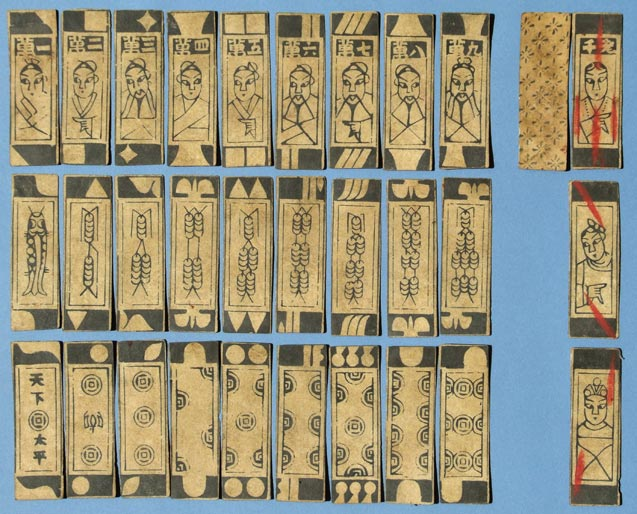
\includegraphics[width=0.75\textwidth]{1_shihu.jpg}
\caption{Niekompletny zestaw do gry w \pinyin{shihu}; 30 spośród 120 kart;
Chiny, ok. 1900 r;  źródło:
http://www.themahjongtileset.co.uk/tile-set-history/earliest-suit-names/}
\end{figure}

% MADIAO
Same karty używane do gry w \pinyin{shihu} wykorzystywane były również do wielu
innych gier, a ich wcześniejszym zastosowaniem prawdopodobnie była gra w
\pinyin{madiao} (馬吊 \pinyin{mǎdiào}), czyli dosłownie ,,wieszanie konia'',
pochodząca z czasu rządów cesarza Kangxi (康熙 Kāngxī), czyli z lat 1661--1722(Jin
1783).
Zestaw \pinyin{madiao} składał się z 40 kart w 4 taliach -- czwarta talia,
niewystępująca w grach wywodzących się z \pinyin{madiao}, nazywana była
,,dziesiątkami myriad''. Później wykorzystywano zestawy zawierające tylko 3
talie (czyli 30 kart) do innych gier.(Stanwick, Xu)

%MOHU
Przykładem innej gry wykorzystującej zestaw do \pinyin{madiao} jest
\pinyin{mohu} (默和 \pinyin{mòhú}). Nazwę \pinyin{mohu} można dosłownie przetłumaczyć jako
,,układanie kart w ciszy''. Gra była przeznaczona dla 4 graczy i wymagała 60
kart (czyli najprawdopodobniej 2 zestawów kart \pinyin{madiao} pozbawionych
talii dziesiątków myriad). Jeden z graczy rozdawał wszystkim uczestnikom po
kolei po 1 karcie, aż każdy miał ich po 10. Następnie gracze układali je w
ciszy. Dalsza rozgrywka polegała na dobieraniu kart z pozostałych 20 w celu
ułożenia zwycięskiego układu (jeden z graczy, ale nie ten odpowiadający za
pierwsze rozdanie kart, rozdawał kolejne).(Jin 1783; Stanwick, Xu)
% 
% \footnote{,,Natrafianie na układ z
% kart'' to dosłowne znaczenie nazwy \pinyin{penghu}, jednakże prawdopodobnie jej
% pochodzenie jest nieco inne. \pinyin{Peng} (碰 \pinyin{pèng}) to jedna z
% najczęściej stosowanych deklaracji we współczesnym madżongu. Jej użycie pozwala
% na dobranie kamienia odrzuconego przez innego gracza do własnej trójki takich
% samych kamieni. Prawdopodobnie zachodzi związek pomiędzy tą nazwą, a nazwą gry w \pinyin{penghu}.}


% PENGHU
Inną tego typu grą jest \pinyin{penghu} (碰和 \pinyin{pènghú} -- dosłownie
,,natrafianie na układ z kart'').
W \pinyin{penghu} grano 4 lub 5 zestawami do \pinyin{madiao}, czyli łącznie 120
lub 150 kart. (Stanwick, Xu) Inne źródło sugeruje, że stosowano 2 lub 2,5
zestawu do \pinyin{mohu} (Jin 1783), co sumuje się do tej samej liczby kart. Gra
prawdopodobnie wykształciła się z \pinyin{mohu}. Pojawiają się w niej układy
występujące również we współczesnym madżongu, jak na przykład
\pinyin{peng}\footnote{\pinyin{peng} (碰 \pinyin{pèng}) to jedna z
 najczęściej stosowanych deklaracji we współczesnym madżongu. Jej użycie pozwala
 na dobranie kamienia odrzuconego przez innego gracza do własnej trójki takich
 samych kamieni. Występuje również w grze w \pinyin{penghu} i jest elementem jej
 nazwy.}. Można sądzić, że niektóre źródła mowiące tylko o \pinyin{shihu} lub
 tylko o \pinyin{penghu} nie rozróżniały tych dwóch gier, jako że ich zasady i
 skład zestawów do gry były do siebie zbliżone. (Jin, 1783; Stanwick, Xu)

% PODSUMOWANIE KART
Karty do \pinyin{madiao} były również wykorzystywane do szeregu innych,
pomniejszych gier, jak \pinyin{kanhu} (看虎 \pinyin{kànhǔ} -- ,,obserwowanie
tygrysa''), \pinyin{hunjiang} (混江 \pinyin{hùnjiāng} -- ,,zwijanie rzeki'') oraz
\pinyin{suohu} (梭和 \pinyin{suōhú} - ,,układanie kart ruchem w tę i z
powrotem''). (Stanwick, Xu) Każda z nich jest warta wspomnienia, jako że wielu
pasjonatów oraz badaczy na przełomie XIX i XX wieku określało zestawy do
madżonga właśnie ich nazwami (nie będąc jeszcze świadomym różnicy).
Można wręcz przypuszczać, że funkcjonowały one przez długi czas równolegle z
nowo wykształconym madżongiem, a być może nawet grano w nie w przy pomocy
kamieni zamiast kart.


















